\documentclass[solution, letterpaper]{cs20inclass}
\usepackage{enumerate}
\usepackage{tikz}
\usepackage{pgf}
\usepackage{tikz}
\usepackage{hyperref}
\begin{document}
\header{21}{Friday, March 25, 2016}

\noindent Author: Hannah Blumberg

\paragraph*{Executive Summary}
\begin{enumerate}
  \item \textbf{Connected}. Two vertices are \emph{connected} if there is a path between them. A \emph{connected component} of an undirected graph is a subgraph in which all pairs of vertices are connected by at least one path and which is not connected to any additional vertices in the supergraph. A graph is \emph{connected} if it has only one connected component. 

  \item \textbf{Edge connectivity}. The \emph{edge connectivity} of a graph is the smallest number of edges that must be removed to disconnect it. An edge whose deletion increases the number of connected components is called a \emph{bridge}.  

  \item \textbf{$k$-edge Connectivity}. A graph is \emph{k-edge-connected} if it remains connected whenever fewer than $k$ edges are removed. The edge-connectivity of a graph is the largest $k$ for which the graph is $k$-edge-connected. (In other words, the edge-connectivity of a graph is the smallest number of edges that can be removed to disconnect the graph.)

  \item \textbf{Vertex connectivity}. The \textit{vertex connectivity} of a graph is the smallest number of vertices that can be removed to disconnect the graph. A vertex whose deletion increases the number of connected components is called an \emph{articulation point}.
\end{enumerate}

%% PROBLEM 1 %%
\problem
What are the edge and vertex connectivities of the following graphs?

\subproblem The complete graph $K_n$. (By definition, a complete graph does not have a vertex connectivity by definition. Only give the edge connectivity.)
\subproblem A cycle of length $n$, $C_n$.
\subproblem A path of length $n$ ($n$ vertices), $P_n$.
\subproblem 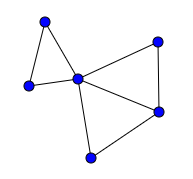
\includegraphics[width=4cm]{class21-1}

\begin{solution}
  \subsolution Edge connectivity: $n-1$, Each node has $n-1$ edges (an edge to every other node). In order to disconnect a node, you must remove all of its $n-1$ edges.

  \subsolution Edge connectivity: 2, If you remove 1 edge, you create a path. If you remove a second edge from the path, it becomes disconnected.

\noindent Vertex connectivity: 2, If you remove 1 vertex, you create a path. If you remove a second vertex from the path, it becomes disconnected.

  \subsolution Edge connectivity: 1

\noindent Vertex connectivity: 1

  \subsolution Edge connectivity: 2, Each vertex has a degree of at least 2. In order to disconnect a vertex, at least 2 edges must be removed.

\noindent Vertex connectivity: 1, If you remove the center vertex (the vertex with degree 5), the graph becomes disconnected.

\end{solution}

%% PROBLEM 2 %%
\problem
Show that ``being connected'' in an undirected graph is an equivalence relation.

\begin{solution}
\begin{itemize}

  \item \textbf{Reflexive}: By definition, all vertices are connected to themselves. (There is a length 0 path from any vertex $u$ to itself.) Therefore, being connected is reflexive.

  \item \textbf{Symmetric}: If vertices $u$ and $v$ are connected, then there is a path from $u$ to $v$. Since the edges in the graph are undirected, there is also a path from $v$ to $u$. Therefore, $v$ and $u$ are connected, and we can conclude that being connected is symmetric.

  \item \textbf{Transitive}: Suppose $u$ is connected to $v$ and $v$ is connected to $w$. By definition, there is a path from $u$ to $v$: $u, u_1, u_2,..., u_k-1, u_k, v$ and a path from $v$ to $w$: $v, v_1, v_2, ..., v_n-1, v_n, w$. Then there is a path from $u$ to $w$: $u, u_1, u_2,..., u_k-1, u_k, v, v_1, v_2, ..., v_n-1, v_n, w$. Therefore, $u$ and $w$ are connected, and we can conclude that being connected is transitive.

\end{itemize}

\noindent Since being connected is reflective, symmetric, and transitive, it is an equivalence relation.
\end{solution}

%% PROBLEM 3 %%
\problem 
\textit{(Adapted from a question by former CS20 TF, Corinne Curcie.)}

\noindent Corinne is writing Harry Potter fan-fiction. To get a lot of readers, her stories inevitably end up with a large network of relationships. The following is a graph showing relationships from Corinne's latest fan-fiction, \emph{The Dementor's Kiss}. 

\medskip

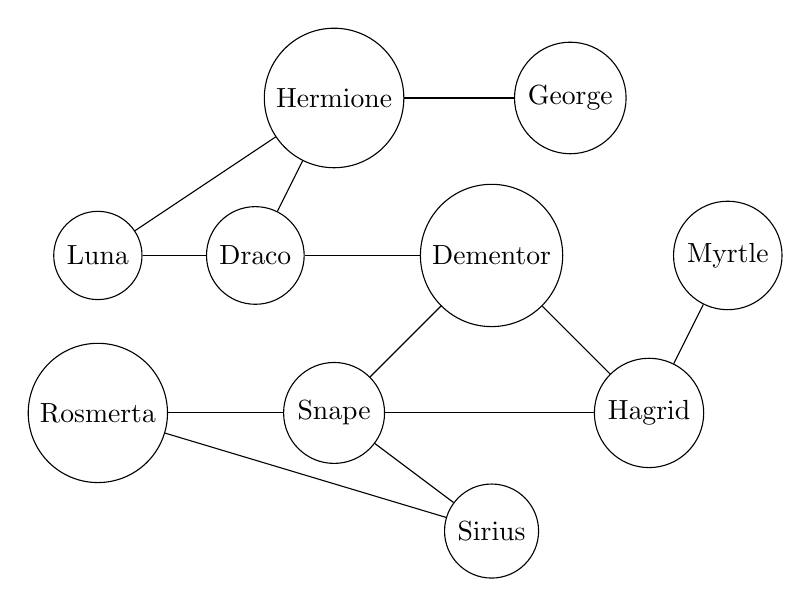
\begin{tikzpicture}
\node (1) at (1,0) [shape = circle, draw] {Snape};
\node (2) at (3, -1.5) [shape = circle, draw] {Sirius};
\node (3) at (3, 2) [shape= circle, draw] {Dementor};
\node (4) at (1,4) [shape= circle, draw] {Hermione};
\node (5) at (0,2) [shape = circle, draw] {Draco};
\node (6) at (-2,2) [shape = circle, draw] {Luna};
\node (7) at (4,4) [shape = circle, draw] {George};
\node (8) at (6,2) [shape = circle, draw] {Myrtle};
\node (9) at (5,0) [shape = circle, draw] {Hagrid};
\node (10) at (-2,0) [shape = circle, draw] {Rosmerta};

\path [-] (1)edge (2);
\path [-] (6)edge  (4);
\path [-] (1)edge (3);
\path [-] (3)edge (5);
\path [-] (4)edge (5);
\path [-] (5)edge (6);
\path [-] (4)edge (7);
\path [-] (1)edge (9);
\path [-] (3)edge (9);
\path [-] (8)edge (9);
\path [-] (1)edge (10);
\path [-] (2)edge (10);

\end{tikzpicture}

\subproblem What is the vertex connectivity?
\subproblem What is the edge connectivity?
\subproblem What are the articulation points?
\subproblem What are the bridges that exist?

\begin{solution}
\subsolution 1
\subsolution 1
\subsolution Hermione, Dementor, Hagrid, Snape and Draco are articulation points. 
\subsolution Hermione-George, Draco-Dementor, and Hagrid-Myrtle are bridges.
\end{solution}

%% PROBLEM 4 %%
\problem
(Bonus) Schedule the final exams for the 6 courses --- CS51, MATH21b, CS20, CS179, CS171, and CS124 --- using the fewest number of different time slots. Courses that have students in common cannot be scheduled at the same time, and the following 8 pairs share at least one student: \\

\noindent (CS51, MATH21b), (CS51, CS179), (MATH21b, CS20), (MATH21b, CS171), (CS20, CS179), (CS20, CS171), (CS124, CS179), (CS171, CS124)

\begin{solution}
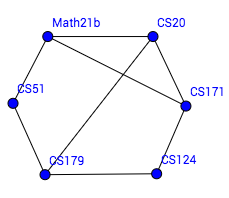
\includegraphics[width=5cm]{class21-2}

\noindent Since CS20, MATH21b, and CS179 all have a student in common, there must be at least three slots. Here is one possible schedule (note that there are several):

\begin{enumerate}
  \item CS20, CS51
  \item MATH21b, CS124
  \item CS179, CS171
\end{enumerate}
\end{solution}
\end{document}